\section{流域水治理演变模式}

研究结果显示黄河流域在人类主导时期有三种不同的流域治理模式:集中供水时期(P1: 1965 \textendash{} 1978)、治理转变时期(P2: 1979 \textendash{} 2001)和适应转向时期(P3: 2002 \textendash{} 2013)(图~\ref{ch4:fig:IWGI})。
在黄河流域水资源压力相对较低的集中供水时期(1965 \textendash{} 1978),主要的水资源需求是为牲畜和作物等提供供给服务,水治理也倾向于通过建造水库和引水渠等来增加水资源供给。
然而,水资源供应的增加并不能促进人\textendash{}水关系和谐,因为它在不考虑生态保护的情况下急剧增加了用水,且这往往是一种不可逆转的变化\cite{zhou2020}。
在接下来的十年内,灌溉农田和引水设施的迅速扩张使黄河流域超负荷取水。
1972年以来,超过$80\%$的地表水被使用,导致河流频繁枯竭,造成了额外的生态问题,如湿地萎缩和生物多样性下降\cite{wang2019c, fu2021}。
此外,由于继续增加供应是不切实际的,水资源压力限制了新兴的、更有利可图的工业与服务业的发展,流域的水治理模式接近了社会-生态危机的临界点\cite{loch2020, wohlfart2016}。

治理体制转型时期的开始(P2: 1979 \textendash{} 2001)恰逢“改革开放”后,水资源竞争的持续加剧,但枯竭的黄河已经开始断流。
黄河流域在此时期开始经历水治理转变,这一结果与理论分析的结果高度一致:在流域总供应稳定的情况下,水资源需求在接近可供给水资源上限后的持续增长,将为流域水治理带来重大转型,流域社会\textendash{}水文系统将通过制度措施快速增强社会适应力,以响应该水资源供小于求的临界点\cite{loch2020}。
因此黄河流域在此时期采取了诸多水治理举措,包括控制灌溉面积的增长、倡导节水设施建设、制定全国首个水资源配额制度、并初步制定跨流域调水方案(南水北调)等\cite{wang2019b,long2020,nickum2021},成为了中国九大流域的制度变革先驱。
因此,尽管黄河流域的水资源压力仍然很大,且因径流减少和用水灵活性降低而持续增加,但黄河的断流问题却得到了解决,$1999$年的最后一次断流昭示着此次水治理转变的巨大影响\cite{wang2019b}。
许多地区在此时期发生了产业结构转型,内蒙古的重工业,如煤炭和钢铁等行业,对水资源的需求量非常大,使用水的方式和量也很特殊,如在生产过程中需要大量用水进行冷却和清洗,同时产生的废水也需要进行处理,这些行业对水的需求对当地水资源的管理和保护带来了挑战。

在随后的适应增强时期(P3: 2002 \textendash{} 2013)为适应稳定在高位的水资源压力,许多国家层面的黄河流域水治理实践都在这一时期提出,以期用最经济的方式,在保护生态的同时实现流域高质量发展。
二十一世纪初提出的“环境整治”和$2011$年提出的“最严格水资源管理”都是对水资源粗放式开发利用的响应,不断使流域水治理模式变得更高效。
这一时期除了中央政府主导的适应举措,地区各部门之间为了追求生产效率,社会经济过程为“水使用目的、水分配方式”的权衡发挥了重要作用。
典型的例子是黄河流域的水权转换工作,许多地区都积极推动了农业节水转型,并将节约的水额供给到经济效益更高的工业服务业之中。
通过不同行业和地区对流域水资源的广泛重建,通过日益强化的社会-经济过程调整以前粗放的发展模式以及刚性的制度约束,这些都是水治理适应性增强的体现,以此在有限的供水条件下优化平衡来自不同地区、不同行业的需求\cite{dalin2015,song2022}

\begin{figure}[!ht]
	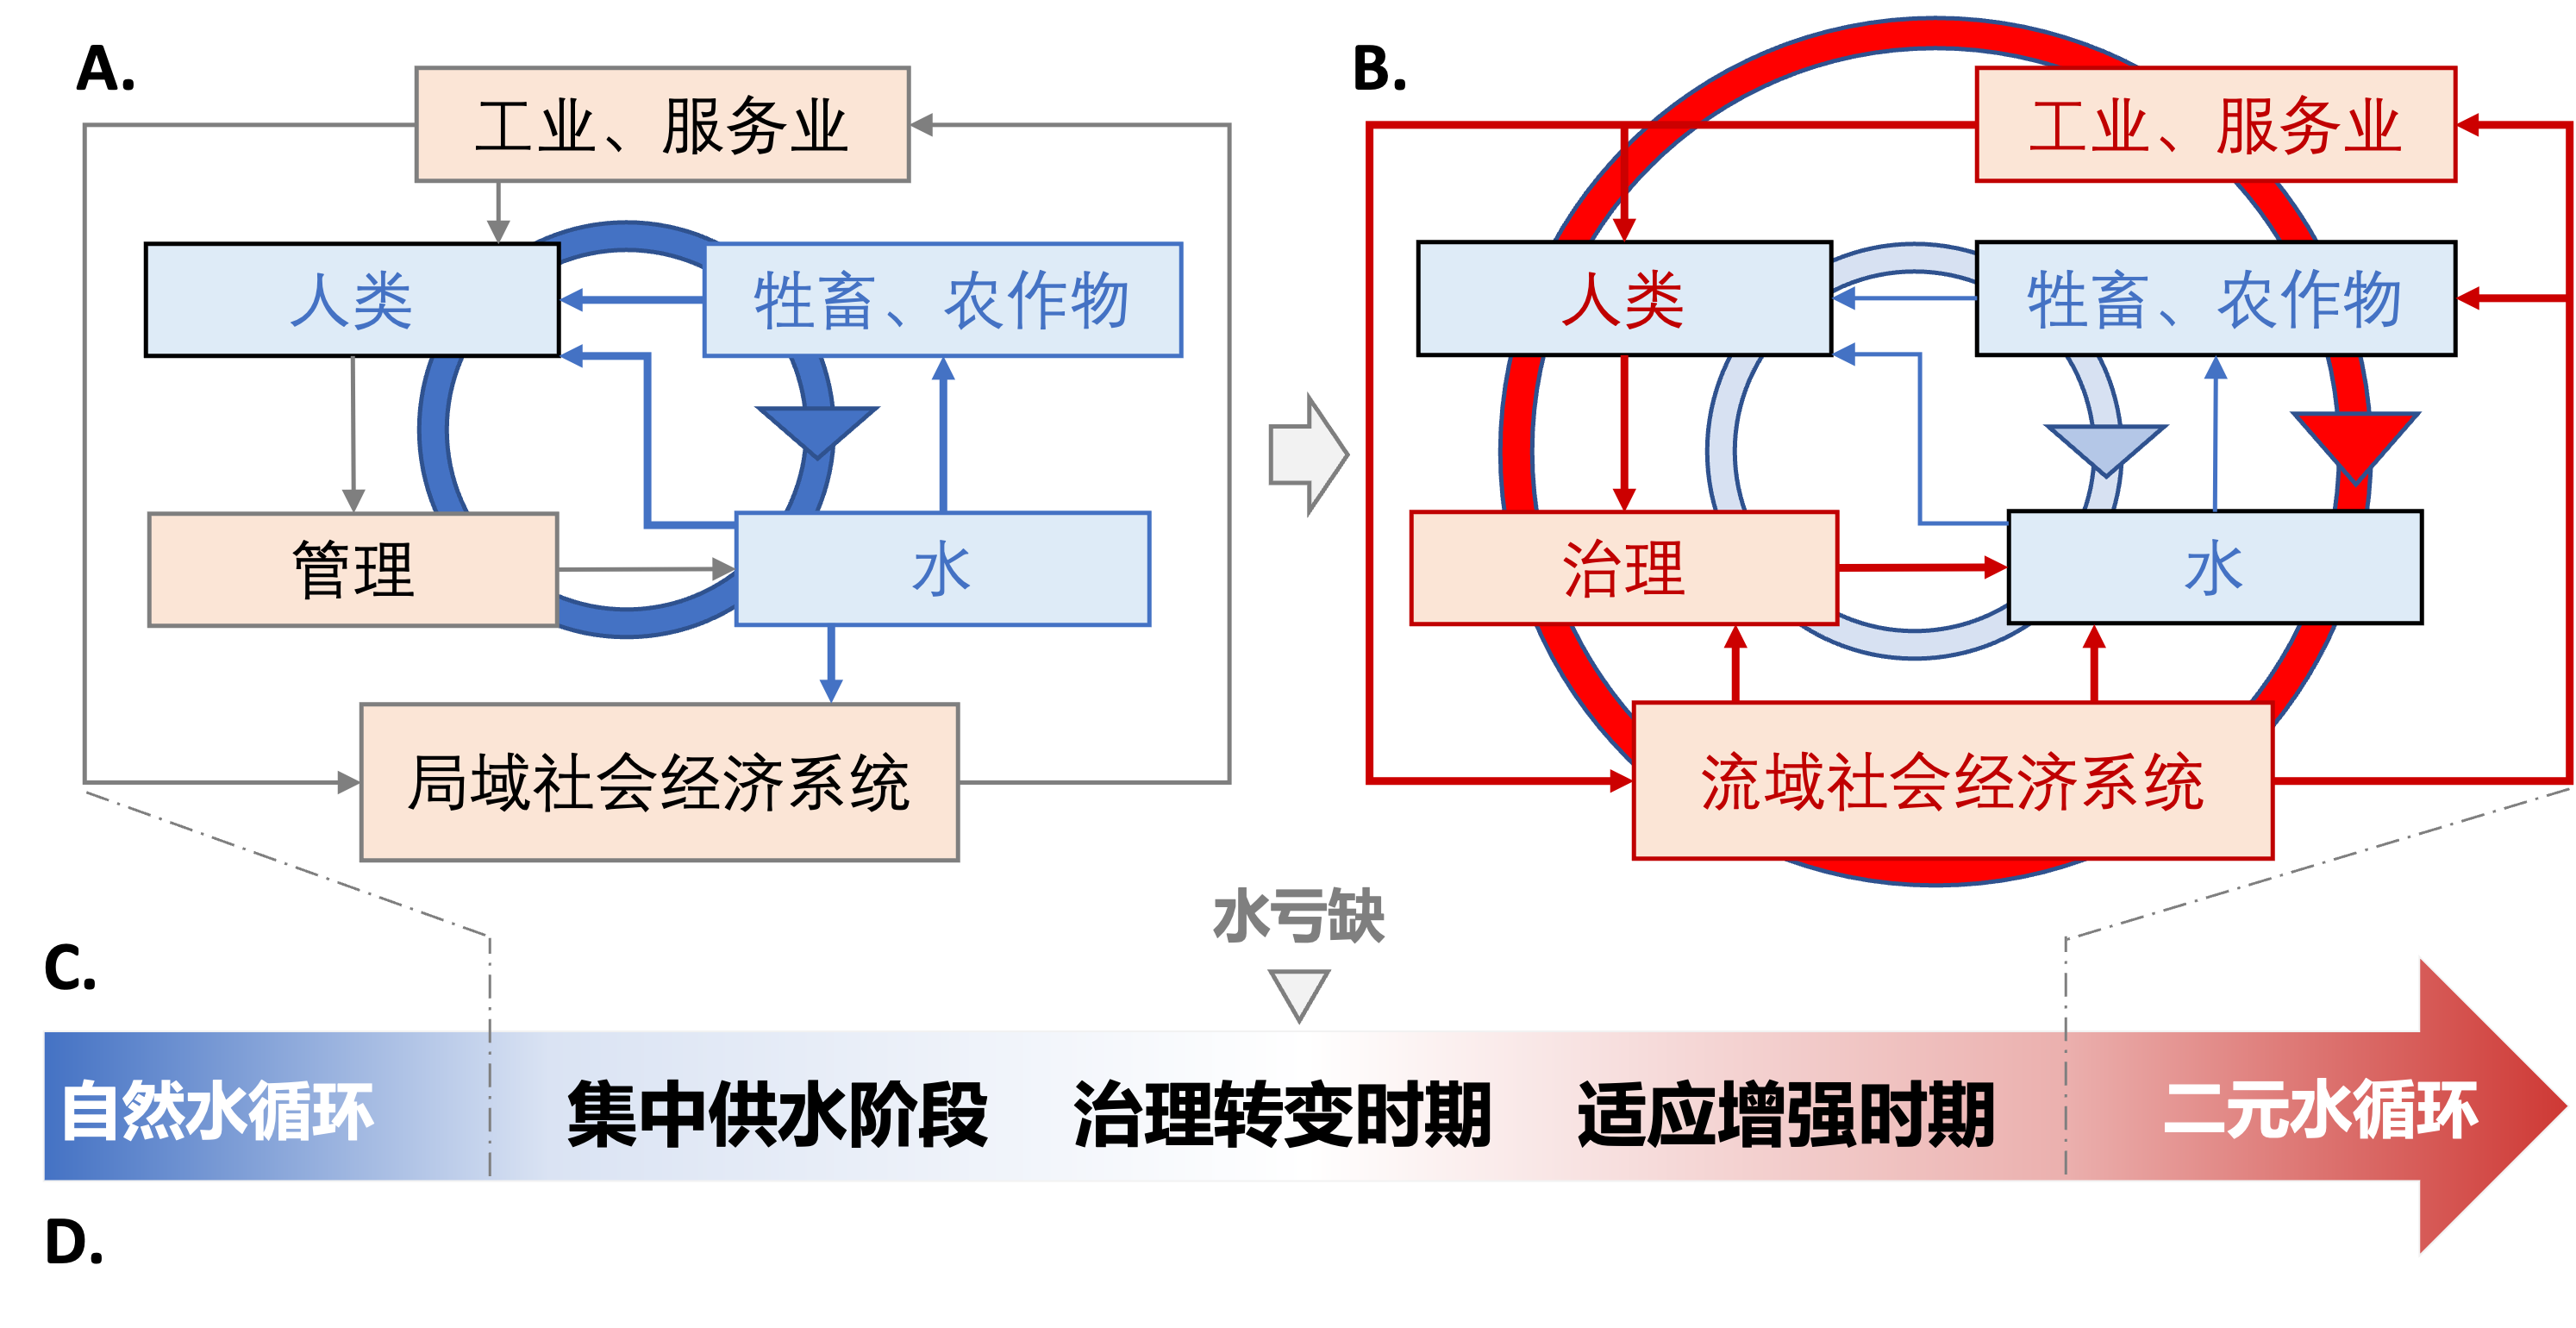
\includegraphics[width=\textwidth]{img/ch4/ch4_transition.png}
	\caption[人类主导下流域系统的水治理阶段过渡]{
		人类主导下流域系统的水治理变化过程。蓝色代表人类活动尚未成为主导的社会\textendash{}水文循环,红色代表由社会经济过程主导的流域水过程。
        \textbf{A.}随着社会经济系统的发展,用以非供给服务的水需求增加;同时,通过水库等工程措施使人们能够控制水循环并局部缓解水资源压力。
        \textbf{B.}随着人为干预升级,不同地区和部门间的用水权衡愈发突出;流域亟需提升利用效率和调度能力,并组织起更具适应性的水治理。
        % \textbf{C.}在人类主导的流域社会\textendash{}水文循环模式下,水治理转变常发生在水资源亏缺之后,在社会-经济过程主导下推动适应能力快速增长。在此之前水治理主要面临经济和环境挑战,但随后面临社会和政策挑战。
	}\label{fig:summary}
\end{figure}

黄河流域的水治理演化过程是“增大供给、治理转变、适应增强”的突出的案例,而其中变化的内在机制已在全球由人类主导流域社会-水循环的过程中广泛出现(图~\ref{fig:summary})。
图~\ref{fig:summary}~A和B中的大循环箭头示意不同时期主导的社会、水文过程,其中A图所示的阶段由水文循环主导,B中则由社会-经济过程主导。
供给性用水(包括图~\ref{fig:summary}中人类、牲畜、农作物用水),以及非供给性的工业、服务业的用水与自然\textendash{}社会二元水循环的关系如图所示,灰色粗箭头代表量比较少,红色箭头表示更重要。
为了支持早期的区域社会经济系统用水,流域治理策略倾向于为了维系水循环的稳定而管理自然水过程。
在图~\ref{fig:summary}~B所示的阶段开始强调在全流域范围内进行水资源调度,由逐渐增强的社会经济系统的需求调整水治理策略,并适应性地进行水治理。

在人类主导的流域社会\textendash{}水文循环模式下,水治理转变常发生在水资源亏缺之后,在社会-经济过程主导下推动适应能力快速增长。
随着社会-经济过程对水循环影响加深,不同时期的流域面临不同的水治理挑战:在前期主要是经济和环境方面,在后期集中于与制度和政策方面。
放眼全球其它流域,以水资源短缺和供水困难为代表的水治理挑战是制约发展中流域的瓶颈\cite{allan2019,speed2013,liu2012}。
人类社会-经济过程主导的发达流域(特别是跨界河流)则须重点解决结构性挑战,如水纠纷或缺乏公平\cite{mirumachi2015}。
本章研究开发并使用的综合水治理指数(IWGI)可以将流域水治理变化过程与这些挑战联系起来,提供了一种解释人类活动主导下人\textendash{}水关系变化的方法。

\section{人\textendash{}水关系变化带来的流域治理挑战}

通过在数据丰富的黄河流域应用综合水治理指数(IWGI),本章研究表明所有的水治理问题都会导致“谁获得水、何时获得水以及如何获得水”的改变,因此监测“稀缺情况、使用目的、分配方式”三个关键问题对识别流域水治理变化有极大帮助。
但在世界范围内广泛应用该方法的主要局限是缺乏全球尺度的长时间序列数据,这意味着IWGI的可能缺点是难以推广。
在数据相对不足的流域应用IWGI时,建议不同方面的指标选择可根据现有数据集进行调整,因为底层指标之间关系的变化趋势比精确计算指标更重要。
在当今这个“人类世”,人\textendash{}水关系由人类活动所主导的情况越来越普遍,应对层出不穷的治理挑战已成为复杂的人\textendash{}水系统的核心\cite{cumming2018,cumming2014,jaeger2019}。
许多流域仍在不断接近系统随时可能崩溃的“地球界限”\cite{gleeson2020, wang-erlandsson2022},只有更深入地理解流域水治理系统,结合非线性稳态变化和转型的思想,才能维持流域社会\textendash{}生态系统的弹性并实现可持续、高质量发展\cite{falkenmark2019}。

% Implications
由于大型河流流域是生态系统服务、经济发展和人类福祉的关键来源,水治理逐渐从主要的区域问题成为流域问题或国家问题\cite{best2019,best2020}。
随着联系日益紧密的世界中出现越来越多的水治理挑战,水治理的稳态转变过程反映了社会如何通过增强其在水社会循环中的适应能力来改变治理实践的建议,而IWGI定量地确定了这一转变\cite{loch2020,turton1999,diaz2019}。
科学家和决策者认识到不断变化的治理挑战是至关重要的,因为在一个阶段下开发的模型、制度、工程和方法不一定适用于另一个治理阶段\cite{reyers2018}。
